\documentclass[acus]{JAC2003}

%%
%%  This file was updated in April 2009 by J. Poole to be in line with Word tempaltes
%%
%%  Use \documentclass[boxit]{JAC2003}
%%  to draw a frame with the correct margins on the output.
%%
%%  Use \documentclass[acus]{JAC2003}
%%  for US letter paper layout
%%

\usepackage{graphicx}
\usepackage{booktabs}
\usepackage{url}
\usepackage[colorlinks,linkcolor=blue,anchorcolor=blue,citecolor=blue]{hyperref} % hyper reference to contents 
\usepackage{algorithm,algorithmic}
\usepackage{tikz}
\usepackage{pgflibraryshapes}  
\usepackage{textcomp}

\newcommand{\opal}{\textsc{OPAL}}
\newcommand{\opalt}{\textsc{OPAL-t }}
\newcommand{\opalcycl}{\textsc{OPAL-cycl}}
\newcommand{\opalmap}{\textsc{OPAL-map }}
\newcommand{\opalenv}{\textsc{OPAL-envelop}}

\newcommand{\mad}{\textsc{mad }}
\newcommand{\madnine}{\textsc{mad9 }}
\newcommand{\madninep}{\textsc{mad9p }}
\newcommand{\madeight}{\textsc{mad8 }}

\newcommand{\classic}{\textsc{classic }}
\newcommand{\hfifepart}{\textsc{H5Part }}
\newcommand{\hfifefe}{\textsc{H5FED }}

\renewcommand{\epsilon}{\varepsilon} 
\renewcommand{\vec}[1]{{\bf #1}} 
\newcommand{\dt}[1]{\frac{\partial #1}{\partial t}}
\newcommand{\dtt}[1]{\frac{\partial^2 #1}{\partial t^2}}
\newcommand{\dtvec}[1]{\frac{\partial {\mathbf #1}}{\partial t}}
\newcommand{\dttvec}[1]{\frac{\partial^2 {\mathbf #1}}{\partial t^2}}
\newcommand{\rot}{\vec{\nabla} \wedge }
\renewcommand{\div}{\vec{\nabla} \cdot }

\def\vec#1{\mathbf{#1}}
\def\vecg#1{\boldsymbol{#1}}
\def\norm#1{\| #1 \|} 
\def\tr{^{\!\top}}

\def\curl{{\bf curl}\,}
\def\curlp{{\rm curl}_p\,}
\def\div{{\rm div}\,}
\def\grad{\nabla}
\def\gradp{\nabla_p}
\def\dotp#1#2{\langle#1,#2\rangle}
\def\eps{\varepsilon}

\newcommand{\mat}[1]{\ensuremath{\boldsymbol{#1}}}
\newcommand{\vect}[1]{\ensuremath{\mathbf{#1}}}
\newcommand{\iprod}[2]{\ensuremath{\langle#1,#2\rangle}}
\newcommand{\abs}[1]{\ensuremath{|#1|}}

\newcommand{\Nedelec}{N\'{e}d\'{e}lec}

\newcommand{\id}[1]{\structure{#1}}

\newcommand {\Co}{{\mathbb{C}}}
\newcommand {\Int}{{\mathbb{Z}}}
\newcommand {\Nat}{{\mathbb{N}}}
%
%
\newcommand {\Hcurl}{{H(\mathbf{curl};\Omega)}}
\newcommand {\Hocurl}{{H_0(\mathbf{curl};\Omega)}}
\newcommand {\Hdiv}{{H(\mathrm{div};\Omega)}}
\newcommand {\Hodiv}{{H_0(\mathbf{div};\Omega)}}
%
\renewcommand {\Re}{{\rm I \kern-2pt R}}
\newcommand{\vc}[1]{\mbox{\boldmath $#1$}}
\newcommand {\RM}[1]{\mathrm{#1}}


\newcommand{\bs}[1]{\mathbf #1}

%%
%%   VARIABLE HEIGHT FOR THE TITLE BOX (default 35mm)
%%

\setlength{\titleblockheight}{38mm}

\begin{document}
\title{The Object Oriented Parallel Accelerator Library (\textsc{OPAL})}
\author{A.~Adelmann, S.~Binder, Ch.~Kraus,\\Y .~Ineichen, T.~Schietinger, Paul Scherrer Institut, CH-5234 Villigen, Switzerland\\
S.~Russel, Los Alamos National Laboratory, Los Alamos, NM 87545, \\
J.J.~Yang China Institute of Atomic Energy, Beijing, 102413, China}

\maketitle

\begin{abstract}
 \opal\ (Object Oriented Parallel Accelerator Library) is a tool for charged-particle optics calculations in accelerator structures and beam lines including space charge, short range wake-fields and coherent synchrotron radiation. Built from first principles as a parallel application, \opal\ admits simulations of any scale, from the laptop to the largest high performance computing (HPC) clusters available today. Simulations, in particular HPC simulations, form the third pillar of science, complementing theory and experiment. In this paper we present numerical and HPC capabilities such as fast direct and iterative solvers together with timings for \opal\ production runs. The application of \opal\ to our PSI-XFEL project will demonstrate the versatile capabilities \opal. Plans for future developments will be discussed.\end{abstract}

\section{AIM OF \opal}
\opal\ \cite{opal} is a tool for charged-particle optics calculations in
accelerator structures and beam lines. 
Using the \mad language with extensions, \opal\ is derived from \madninep \cite{mad9} and is based 
on the
CLASSIC \cite{classic} class library,
which was started in 1995 by an international collaboration.  \ippl (Independent Parallel Particle Layer) \cite{ippl} is
the framework which provides parallel particles and fields using a data parallel ansatz. 
\opal\ is built from the ground up as a parallel application exemplifying the fact that HPC 
is the third leg of science, complementing theory and the experiment. 
HPC is made possible now through the increasingly sophisticated mathematical models and evolving computer power available on the desktop
and in super computer centers. The \opal\ framework makes 
it easy to add new features in the form of new \texttt{C++}~classes. \opal\ in the latest version (1.1.5) comes in the following flavors:
{\bf\opalcycl}\ and {\bf\opalt}\ .
%\begin{itemize}
%\item \opalcycl 
%\item \opalt .
%\end{itemize}
\opalt  tracks particles with time as independent variable and can be used to model beam lines, dc guns, photo guns and complete XFEL's excluding the undulator. 
Collective effects such as space charge (3D solver), coherent synchrotron radiation (1D solver) and longitudinal and transverse wake fields are considered.
When comparing simulation results to measured data, collimators (at the moment without secondary effects) and pepper pot elements are important devices. 
%An illustration
%of the inverse pepper pot image and the resulting density histogram is given in Figure \ref{fig:ppot}.   
%\begin{figure}[htb]
%\begin{minipage}[b]{0.5\textwidth}
%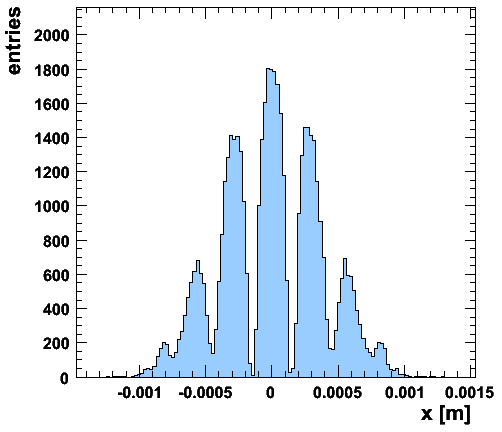
\includegraphics[scale=0.23]{./PepperPotHisto.png}
%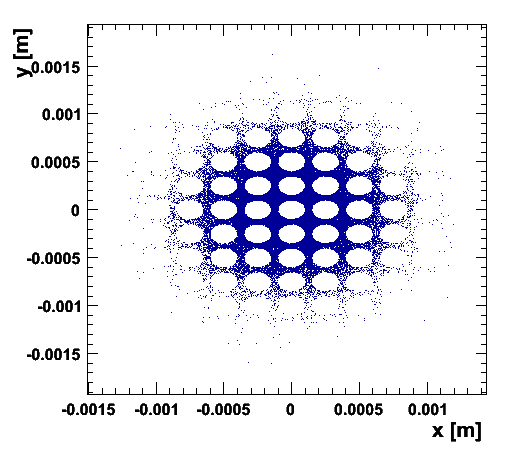
\includegraphics[scale=0.23]{./InversPepperPot.png}
%\end{minipage}
%\caption{Histogram in $x$ (left) of the inverse pepper pot image (right).}
%\label{fig:ppot}
%\end{figure}
\opalcycl is a flavor of \opalt and tracks particles with 3D space charge including neighboring turns in cyclotrons, with time as the independent variable. Both flavors can be used in sequence, hence
full start-to-end cyclotron simulations are possible.  

\section{ARCHITECTURE}
\subsection{A Layered Software Architecture}
\opal\ is based on several external frameworks, it is object oriented, and follows the ideas of design pattern \cite{gammagang}. The data parallel ansatz is provided by  
\ippl (Independent Parallel Particle Layer), the particle accelerator physics is encapsulated in CLASSIC (Class Library for Accelerator Simulation System and Control). The 
parallel I/O is based on \hfifepart \cite{h5part} derived from parallel HDF5. Linear solvers (CG and AMG) are provided by Trilinos \cite{trilinos}. Figure \ref{fig:opalstr} presents a more detailed view into the complex architecture
of \opal. 
\begin{figure}[htb]
\begin{center}
 \begin{tikzpicture}[scale=0.5, transform shape]
    \footnotesize
      \begin{scope}[shape=rectangle,rounded corners,minimum width=3.0cm,minimum height=0.5cm,fill=yellow,text centered]
      
      \draw[rounded corners, draw=green!40, thick, fill=green!25, opacity=0.5, text centered] (-1.55, 1.31) rectangle (8.55,-0.31) node[black, thick, anchor=center, opacity=1., font=\Large] at (3.5, 0.5) {\opal};
      \node[fill= green!40] (0_00) at (0.0,1.0) {MAD-Parser};
      \node[fill= green!40] (0_00) at (3.5,1.0) {Flavors: t,Cycl};
      \node[fill= green!40] (0_00) at (7.0,1.0) {Optimization};
      \node[fill= green!40] (0_00) at (0,0.0)   {Solvers: Direct,MG};
      \node[fill= green!40] (0_00) at (3.5,0.0) {Integrators};
      \node[fill= green!40] (0_00) at (7.0,0.0) {Distributions};

       \draw[rounded corners, draw=red!45, thick, fill=red!25, opacity=0.5, text centered] (-1.55, -0.69) rectangle (8.55,-3.81) node[black, thick, anchor=center, opacity=1.0, font=\Large] at (3.5, -2.25) {\ippl};
       \node[fill= red!45] (q_00) at (0,-1) {FFT};
       \node[fill= red!45] (q_01) at (3.5,-1) {D-Operators};
       \node[fill= red!45] (q_02) at (7,-1) {NGP,CIC, TSI};
       \node[fill= red!45] (q_10) at (0,-1.75) {Fields};
       \node[fill= red!45] (q_11) at (3.5,-1.75) {Mesh};
       \node[fill= red!45] (q_12) at (7,-1.75) {Particles};
       \node[fill=red!45] (q_20) at (0,-2.75) {Load Balancing};
       \node[fill=red!45] (q_21) at (3.5,-2.75) {Domain Decomp.};
       \node[fill=red!45] (q_22) at (7,-2.75) {Message Passing};
       \node[fill=red!45] (q_20) at (0,-3.5) {STL};
       \node[fill=red!45] (q_21) at (3.5,-3.5) {PETE};
       \node[fill=red!45] (q_22) at (7,-3.5) {Polymorphism};

       \node[rotate=90,minimum width=1.7cm,fill=gray] (bla) at (-1.9,0.49){\textcolor{white} {\classic}};
       \node[rotate=90,minimum width=3.15cm,fill= magenta] (bla) at (-1.9,-2.225){\textcolor{white}{H5Part and H5FED}};
       \node[fill=blue!65,minimum width=10.75cm] (q_23) at (3.25,-4.25) {\textcolor{white}{Trilinos}};

      \end{scope}
 \end{tikzpicture}
\caption{The \opal\ software structure}
\label{fig:opalstr}
\end{center}
\end{figure}
\subsection{Basic Equations}
In XFEL's, cyclotrons and beam lines under consideration, the collision between particles can be neglected because typical bunch densities are low.
In the time domain, the general equations of motion of charged particles in an electromagnetic field can be expressed by
\begin{equation}\label{eq:motion}
  \frac{d\bs{p}(t)}{dt}  = q\left(c\mbox{\boldmath$\beta$}\times \bs{B} + \bs{E}\right), \nonumber \\
\end{equation}
where $m_0, q,\gamma$ are rest mass, charge, relativistic factor, $\bs{p}=m_0 c \gamma \mbox{\boldmath$\beta$}$ momentum of a particle respectively, 
$c$ speed of light, $\mbox{\boldmath$\beta$}=(\beta_x, \beta_y, \beta_z)$ normalized velocity vector. In general the electric and magnetic vector fields which depend on the time ($t$) and the position ($\bs{x}$) are
written in abbreviated form as \mbox{ $\bs{B}$ } and \mbox{$\bs{E}$} .

In the absence of collisions, the evolution of the beam's distribution function $ f(\bs {x},c\mbox{\boldmath$\beta$},t)$ can be expressed by a collision-less Vlasov equation:
\begin{equation}\label{eq:Vlasov}
  \frac{df}{dt}=\partial_t f + c\mbox{\boldmath$\beta$} \cdot \nabla_x f +q(\bs{E}+ c\mbox{\boldmath$\beta$}\times\bs{B})\cdot \nabla_{c\mbox{\boldmath$\beta$}} f  =  0, 
\end{equation}
where $\bs{E}$ and $\bs{B}$ include both external applied fields, space charge fields and other collective effects such as geometric and coherent synchrotron wake fields
\begin{eqnarray}\label{eq:Allfield}
  \bs{E} & = & \bs{E_{\RM{ext}}}+\bs{E_{\RM{sc}}}+\bs{E_{\RM{wake}}}, \nonumber\\    
  \bs{B} & = & \bs{B_{\RM{ext}}}+\bs{B_{\RM{sc}}}+\bs{B_{\RM{wake}}}.
\end{eqnarray}
The external electromagnetic fields are given by means of field maps or by analytic models. 

The space charge fields can be obtained
by a quasi-static approximation. In this approach, the relative motion of the particles is non-relativistic in the beam rest frame, such that the self-induced magnetic field 
can be neglected. The electric field is computed by solving Poisson equation
\begin{equation}\label{eq:Poisson}
  \nabla^{2} \phi(\bs{x}) = - \frac{\rho(\bs{x})}{\varepsilon_0},
\end{equation}
where $\phi$ and $\rho$ are the electrostatic potential and the spatial charge density in the beam rest frame. The electric field can then be calculated using $ \bs{E}=-\nabla\phi$.
%\begin{equation}\label{eq:Efield}
%  \bs{E}=-\nabla\phi.
%\end{equation}
It is then transformed back to the lab frame by means of a Lorentz transformation yielding both the electric and the magnetic fields as required in Eq.\,(\ref{eq:Allfield}).

The combination of Eq.\,(\ref{eq:Vlasov}) and Eq.\,(\ref{eq:Poisson}) constitutes the Vlasov-Poisson system. 
In the following, we describe the methods of solving these equations using PIC methods.
\subsection{A Direct FFT Based Poisson Solver}
In our implementation of the PIC method, firstly a rectangular 3D grid containing all particles is constructed.  Subsequently, the charges 
are interpolated onto the grid points. Then the discretized Poisson equation is solved on the grid to obtain the scalar field at the grid points. 
The electric field is calculated on the grid and interpolated back on to the positions of the particles .

In \opal\ the discretized Poisson equation is either solved by a combination of a Green function and FFT or by a conjugate gradient algorithm, preconditioned
with algebraic multi-grid using smoothed aggregation (SA-AMG PCG). This 3D solver has the unique capability to include the exact
boundary geometry. %\cite{Hockney:1} 

%At each time step, in order to solve for the space charge fields, the frames $\bs{S}_{\RM{local}}$ and $\bs{S}_{\RM{beam}}$ are redefined according to current 6D 
%phase space distribution, and all particles are transformed from $\bs{S}_{\RM{lab}}$ to $\bs{S}_{\RM{local}}$.
%Then a Lorentz transformation is performed to transform all particles to $\bs{S}_{\RM{beam}}$.
%The Poisson equation is then solved in the frame $\bs{S}_{\RM{beam}}$. 
In 3D Cartesian coordinates, the solution of the Poisson equation at point $\bs{x}$ can be expressed by 
\begin{equation}\label{eq:Poten}
  \phi(\bs{x})= \frac{1}{4\pi\varepsilon_0}\int{G(\bs{x},\bs{x}')\rho(\bs{x},\bs{x}')d\bs{x}'}
\end{equation}
with $G$ the 3D Green function 
\begin{equation}\label{eq:Green}
  G(\bs{x},\bs{x}')= \frac{1}{\sqrt{(\bs{x}-\bs{x}')^2}}
\end{equation}
assuming open boundary conditions.
The typical steps of calculating space charge fields using the Hockney's FFT algorithm is sketched in Algorithm \ref{alg1:sc3d},
where the quantities with superscript $D$ (discrete) refer to grid quantities.

\begin{algorithm}
  \caption{3D Space Charge Calculation} 
  \label{alg1:sc3d}
  \begin{algorithmic}[1]
    \STATE \textbf{procedure} 3DSpaceCharge(In: $\rho$, $G$, Out: $\bs{E_{sc}}$,$\bs{B_{sc}}$)
       \STATE Create 3D rectangular grid which contains all particles, % and doubled it in each dimension, 
       \STATE Interpolate the charge $q$ of each macro-particle to nearby mesh points to obtain $\rho^D$, 
       \STATE Lorentz transformation to obtain $\rho^D$ in the beam rest frame $\bs{S}_{\RM{beam}}$,
       \STATE FFT $\rho^D$ and $G^D$ to obtain $\widehat{\rho}^D$ and $\widehat{G}^D$,
       \STATE Determine $\widehat{\phi}^D$ on the grid using $\widehat{\phi}^D = \widehat{\rho}^D \cdot \widehat{G}^D$,
       \STATE Use FFT$^{-1}$ of $\widehat{\phi }^D$ to obtain $\phi^D$,
       \STATE Compute $\bs{E}^D= -\nabla \phi^D$,
       \STATE Interpolate $\bs{E}$ at the particle positions $\bs{x}$ from $\bs{E}^D$,
       \STATE Perform Lorentz back transform to obtain $\bs{E_{\RM{sc}}}$ and $\bs{B_{\RM{sc}}}$ in  frame $\bs{S}_{\RM{local}}$ and transform back  to $\bs{S}_{\RM{lab}}$.
       \STATE \textbf{end procedure}
  \end{algorithmic}
\end{algorithm}

The image charge of a beam near a cathode is not negligible, hence
open boundary conditions are not justified in such a case. To find the space-charge forces on the beam from
the image charge by the standard Green function method,
we need to solve the Poisson equation with a computational
domain containing both the image charge and the beam.
We are using a shifted-Green function \cite{shgreen} technique in order to efficiently compute the correct potential at the cathode.
With this technique, the FFT is used to calculate the cyclic convolution
and the previous algorithm can be used to calculate the
potential in the shifted field domain.

At  emission from a dc gun, or when calculating neighboring turns in a cyclotron, the electrostatic approximation is not valid anymore. To overcome this problem
we divide the beam into $n$ energy bins. The space charge solve step, has now $n$ separate Lorentz transformations. 
\subsection{Parallel Scalability}
Typical timings for a production run setup of \opal\ are shown in Figure \ref{scalability} on a Cray XT3. 
In this test, 1\,million particles (Gaussian distributed) are used to track 200 time steps in the PSI Injector\,II cyclotron. The grid size is $64 \times 64 \times 64$ which is decomposed onto a two dimensional grid of processors. All the intermediate phase space data is dumped into 
a single \hfifepart file. The dynamic load balancing frequency as well as the phase space dumping frequency are set to modulo 10 of the time step.
\begin{figure}[ht!]
%  {\includegraphics[width=8cm,trim=0cm 0cm 0cm 0cm]{Timing64mesh}}
\includegraphics[width=.7\linewidth]{Timing64mesh}
  \caption{Wall time as a function of processors for a production run setup}
  \label{scalability}
\end{figure}
The computational kernels of \opal\ scales very well up to several thousands of processors and will be discussed in detail in forthcoming papers. 
%\subsection{An AMG-PCG Poisson Solver}
\vspace{-3.5mm}
\section{APPLICATIONS}
\subsection{Code Benchmarking}
We have carefully benchmarked the code against IMPACT-T and found very good agreement. The following elements where compared: emission including energy binning, standing and 
traveling wave structures, quadrupole and solenoid. The Figure \ref{fig:comp} is representative for the benchmarks and show remarkable
agreement by considering 1D coherent synchrotron radiation in a C-shaped compressor as been foreseen in the PSI-XFEL.  
\begin{figure}[htb]
\begin{center}
%\begin{minipage}[b]{0.5\textwidth}
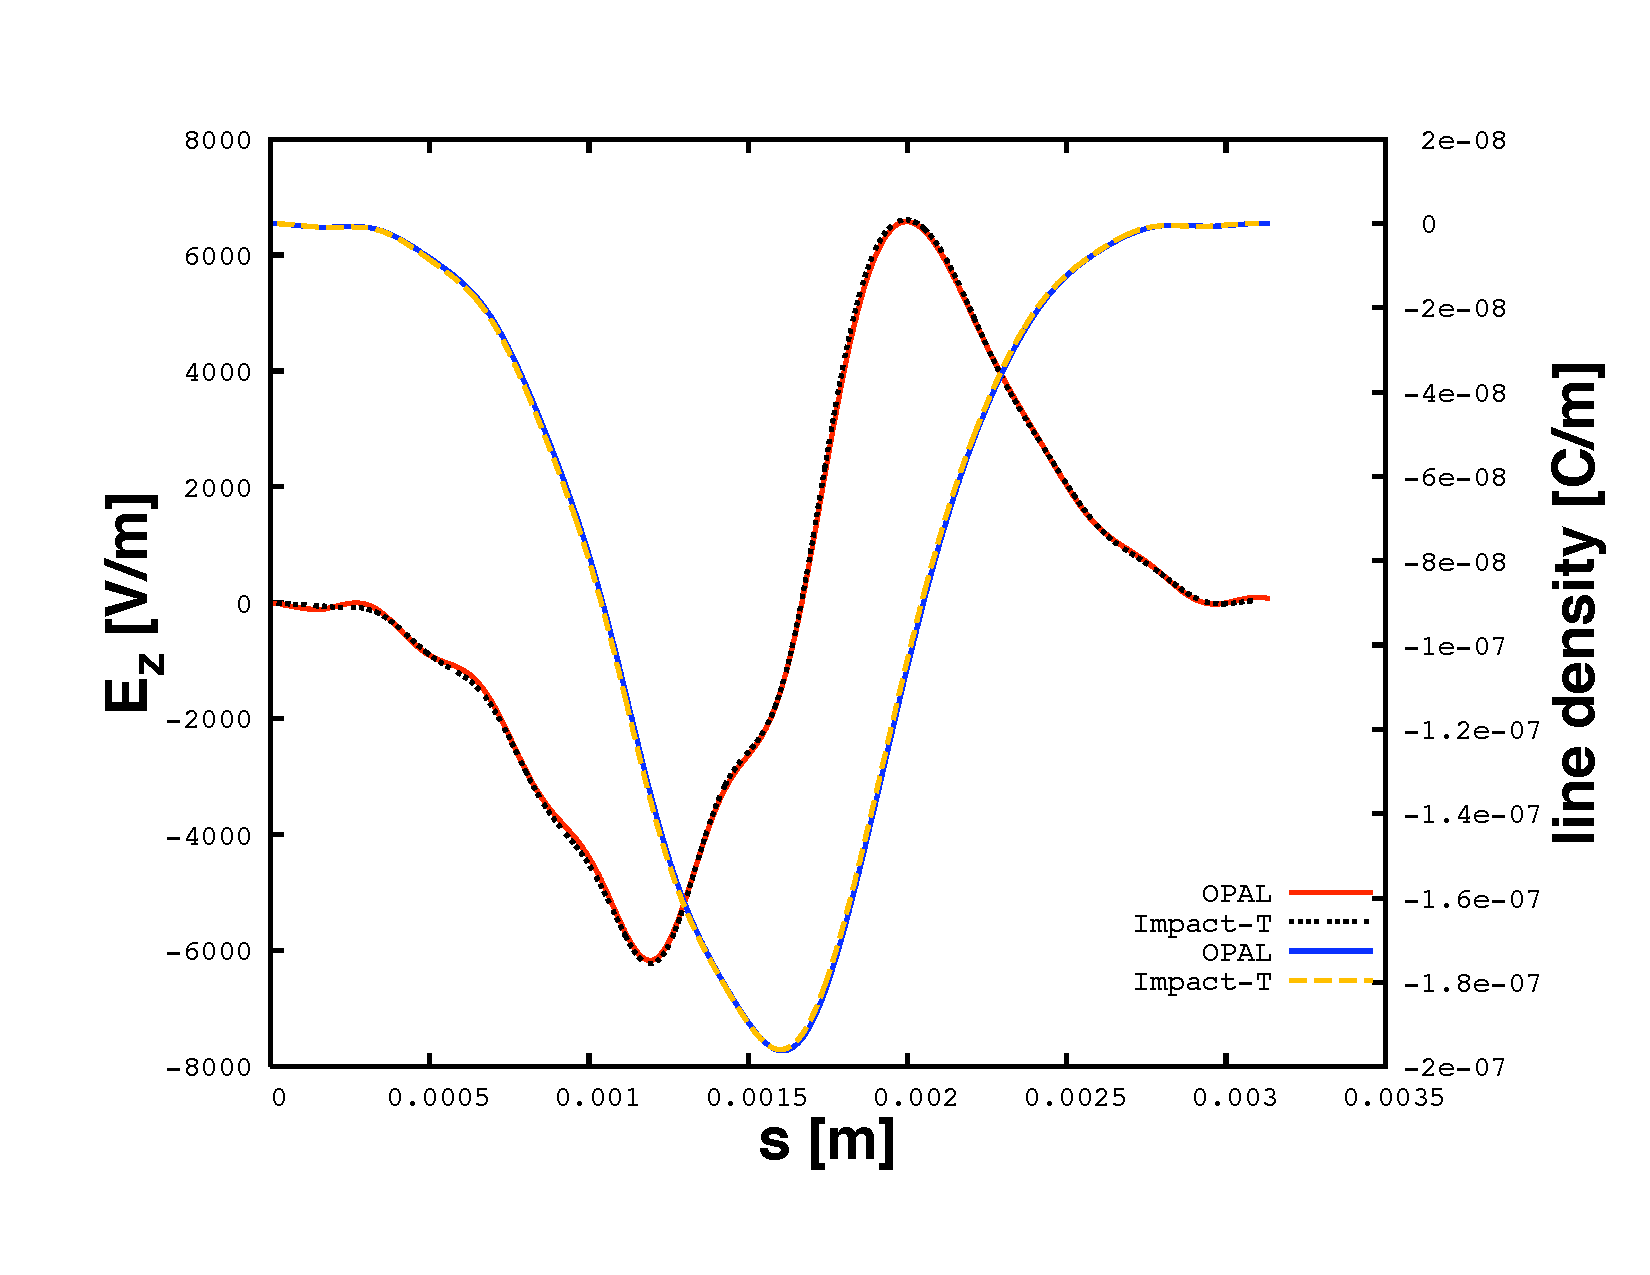
\includegraphics[scale=0.15]{./FR5PFP065-pic1.pdf}
%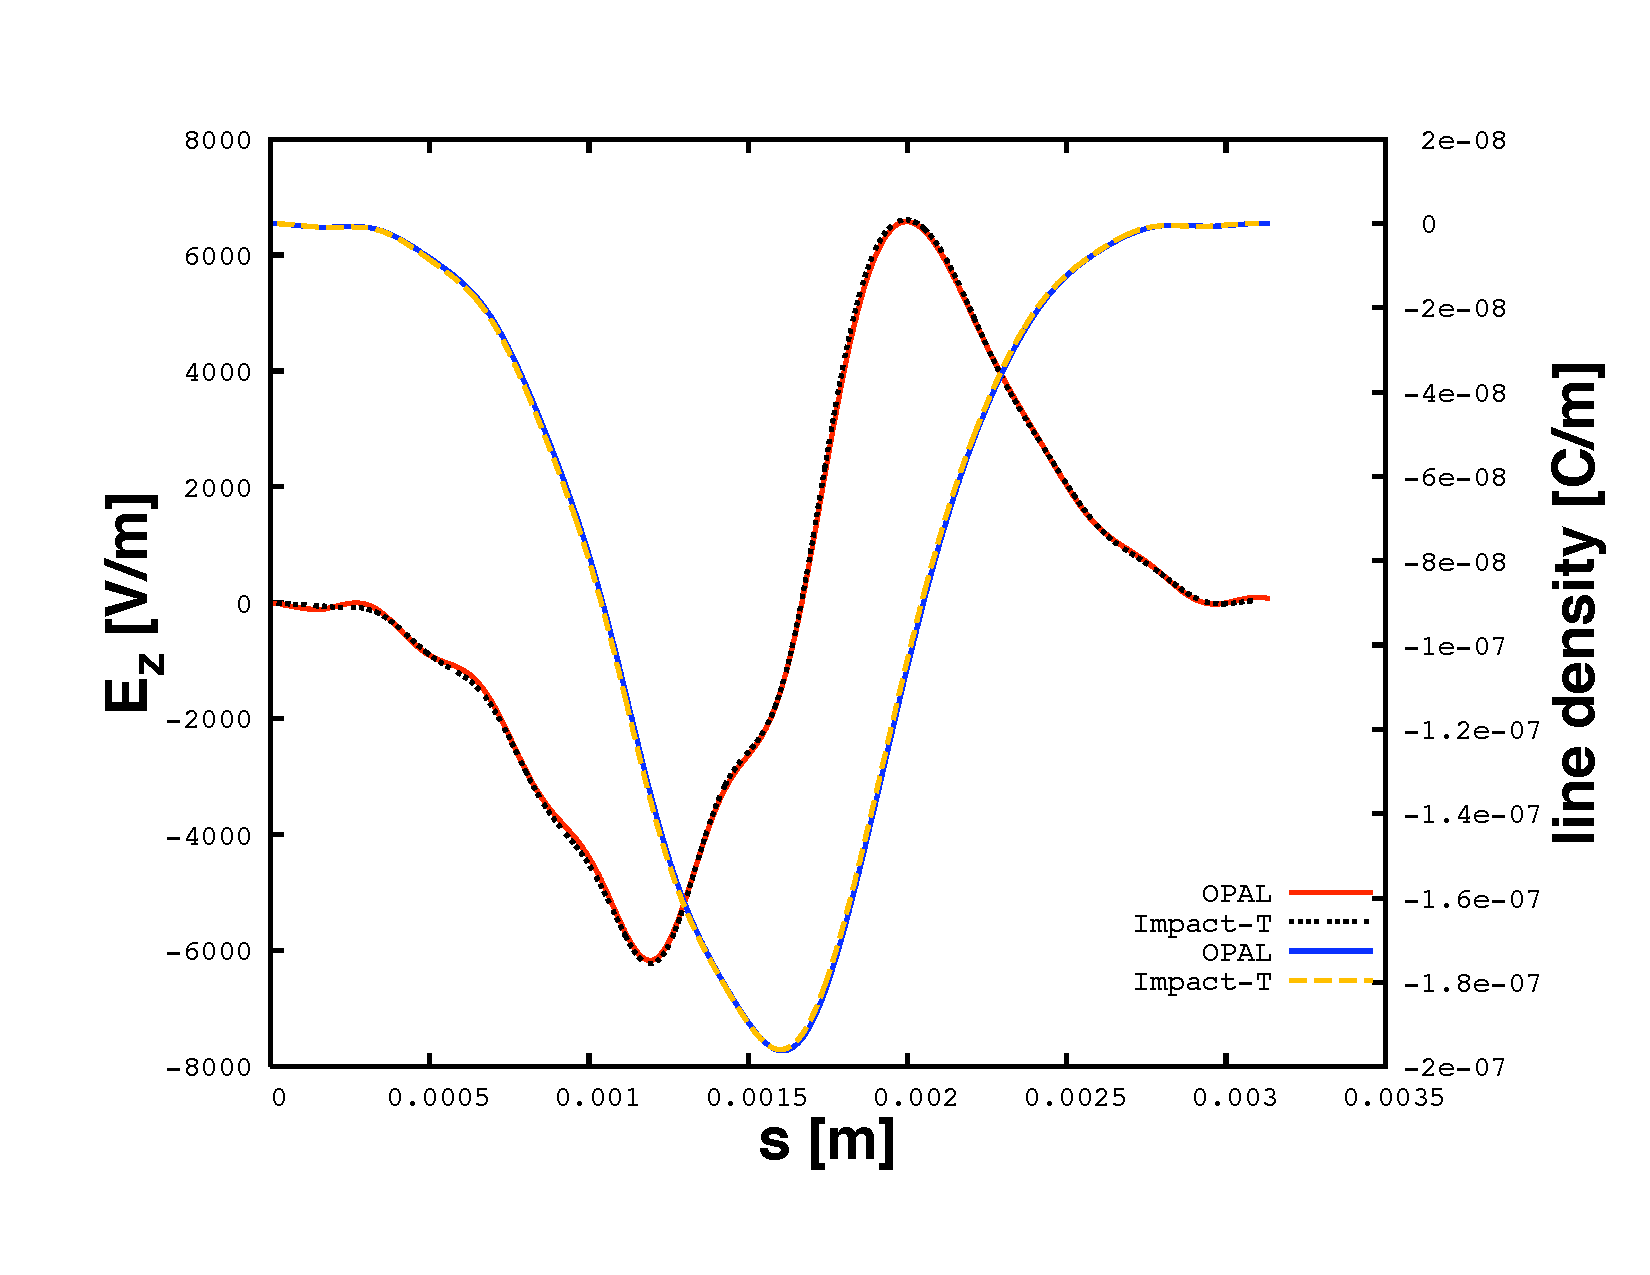
\includegraphics[width=.99\linewidth]{./FR5PFP065-pic1.pdf}
%\end{minipage}
\vspace{-4mm}
\caption{In a C-shaped compressor, the $z$-component of the electric field of a CSR-Wake and the corresponding 1D line density is shown.}
\label{fig:comp}
\end{center}
\end{figure}
\vspace{-4mm}
\subsection{The PSI-XFEL low-emittance electron source}
\opal\ is currently being used to model the low-emittance electron source test stand 
developed and operated in the context of the PSI-XFEL project \cite{obla}.  
The electron gun consists of an adjustable diode configuration subject to pulses of 250~ns (FWHM) 
with amplitude up to 500~kV from an air-core transformer-based high-voltage pulser. 
The facility allows high gradient tests with different cathode configurations and emission processes 
(pulsed field emission and photo emission). 
In the first stage, the beamline consisted of focusing solenoids followed by an emittance 
monitor. 
In Fig.~\ref{fig:comp} we show selected beam characterization measurements from photo cathode operation 
driven by a 266~nm UV laser system delivering 4 \textmu J energy during 6.5~ps (RMS), resulting in 
electron bunches of about 20~pC charge, in comparison to the results of an \opal\ simulation of the same
setup.
The beam sizes are measured with YAG screens, the emittances are estimated with the pepper-pot method
(see Ref.~\cite{obla} for details).

The simulation models the collimating effect of the 1.5 mm diameter anode iris. 
It does not take into account the thermal emittance at the cathode, which may explain the somewhat higher
experimental values.  

The test facility has recently been upgraded with a two-cell RF cavity accelerating the electrons
to an energy of up to 5~MeV.
The upgrade includes various additional diagnostic elements, in particular an energy spectrometer, 
which allows validation of \opal\ tracking in the longitudinal direction.

\begin{figure}[htb]
\begin{center}
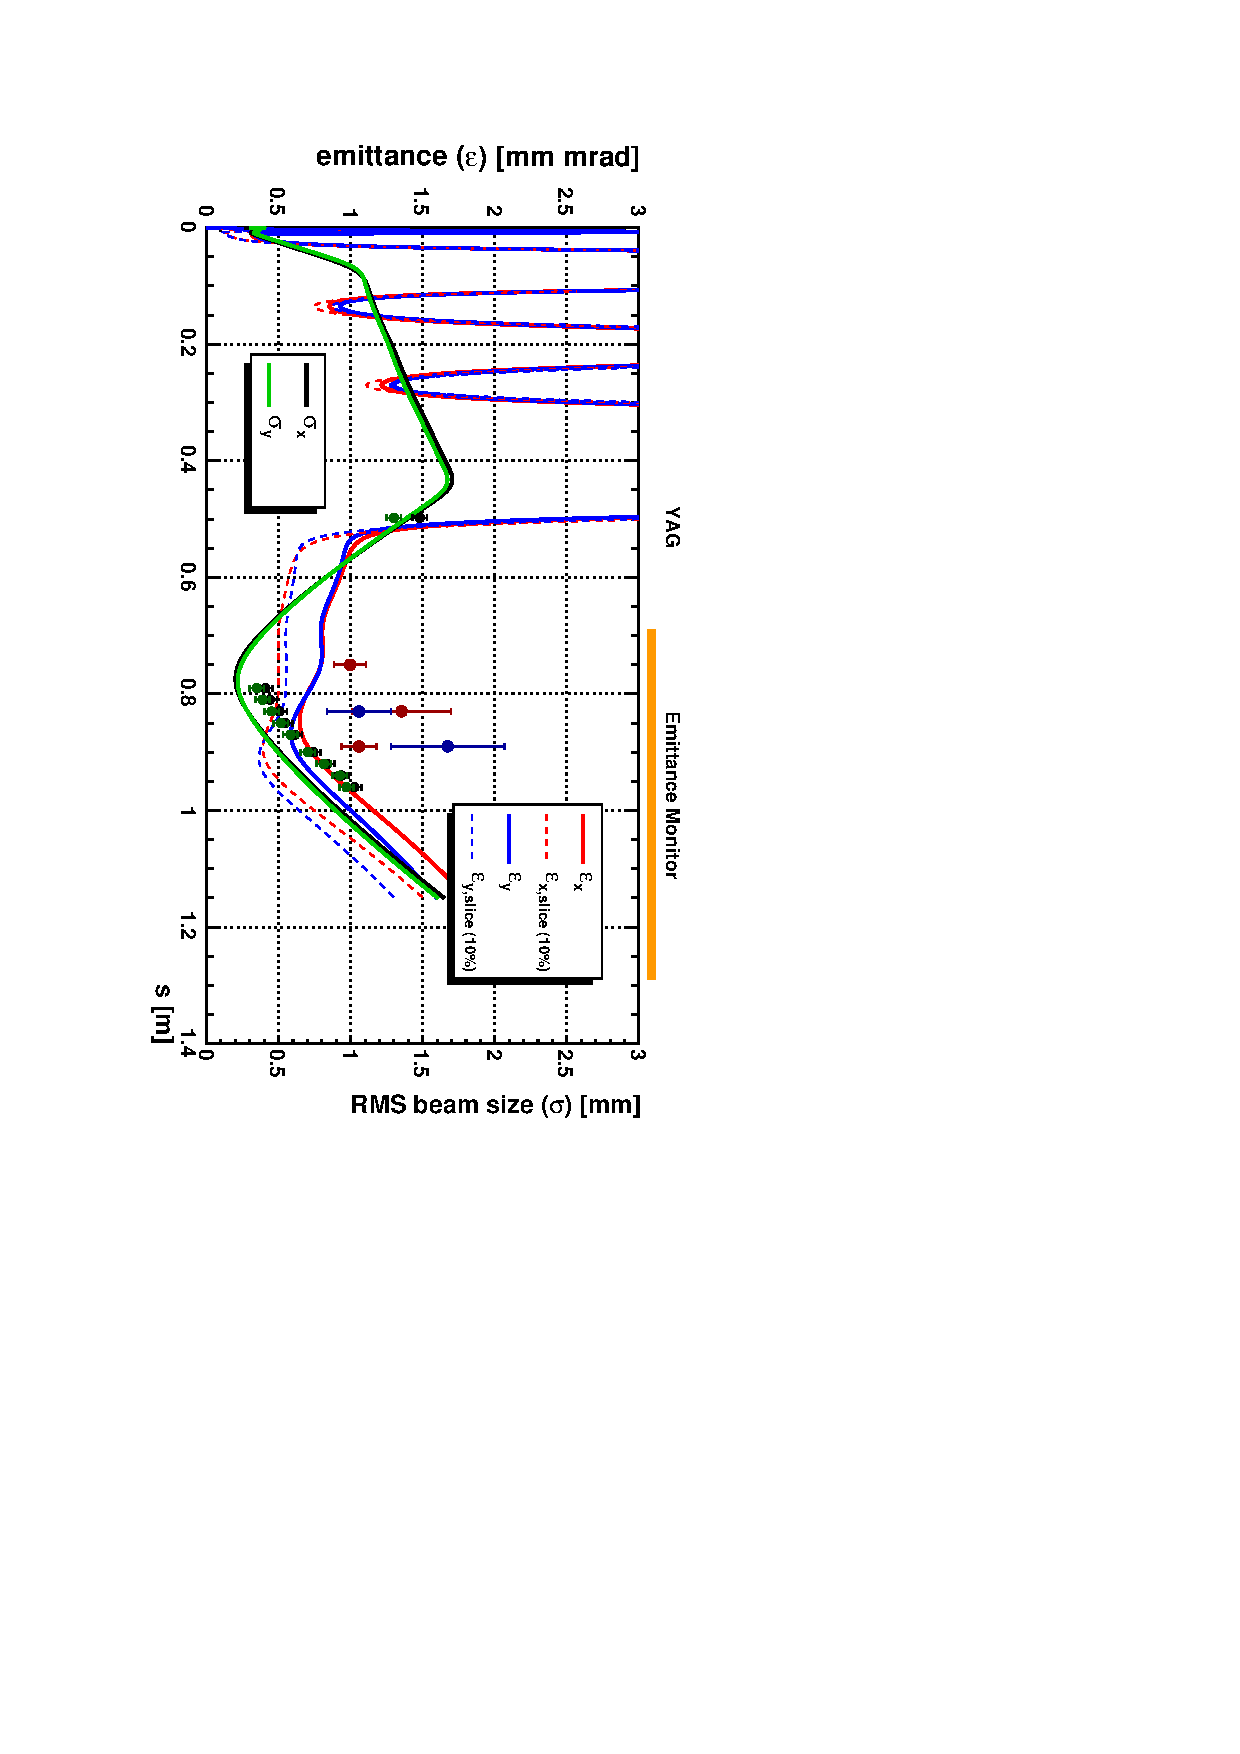
\includegraphics[angle=90,width=.99\linewidth]{./OBLA-Jul22.pdf}
\end{center}
\vspace{-9mm}
\caption{Comparison of \opal\ simulation results (solid and dashed lines) with measurements (points with
error bars). Note that the simulated emittance does not include contributions due to thermal emittance at
the cathode.}
\label{fig:comp}
\end{figure}

%\subsection{The PSI High Intensity Upgrade of the Proton Cyclotrons} 
\vspace{-4mm}
\section{FUTURE PLANS}
Including  two more flavors: 1) \opalmap will track particles with 3D space charge using split operator techniques, and is a proper superset of \madninep \cite{mad9}, and 2)  
a linear space charge mode will become available allowing the user to track moments of the distribution. 
Ongoing  developments towards a 3D finite element time domain Maxwell solver for large structures and simulation capabilities for 3D synchrotron radiation will be included in the more distant future.

This work was partially performed on the Cray XT3 at Swiss National Supercomputing Center (CSCS) within the ``Horizon'' collaboration. 
\begin{thebibliography}{9}   % Use for  1-9  references
%\begin{thebibliography}{99} % Use for 10-99 references
\bibitem{classic} {F. C. Iselin}, {``The CLASSIC Project"}, {Computational Accelerator Physics Conference 1996, Williamsburg, VA.}
\bibitem{mad9}{A. Adelmann and F.C. Iselin and J.M. Jowett and J. Pancin},{ MAD Version 9}, { EPAC 2000},
\bibitem{ippl}{A. Adelmann}, {The \ippl(Independent Parallel Particle Layer) Framework}, PSI-PR-09-05, Paul Scherrer Institut, 2009	
\bibitem{opal}{A. Adelmann, Ch. Kraus, Y. Ineichen and J. J. Yang}, { The \opal\ (Object Oriented Parallel Accelerator Library) Framework}, PSI-PR-08-02, Paul Scherrer Institut, 2008
\bibitem{shgreen} J. Qiang, M. A. Furman and R. D. Ryne, {Phys. Rev. Special Topics - Accel. Beams, 5 (2002) 104402.}
\bibitem{gammagang}{E. Gamma, R. Helm, R. Johnson and J. Vlissides}, {Design Patterns},{Addison-Wesley, ISBN {0201633612}},
\bibitem{h5part}{\em http://h5part.web.psi.ch/}
\bibitem{trilinos} {M.~A. Heroux et.al} { An Overview of the {T}rilinos Project}{ TOMS, {\bf 31}}, {p.397-423}, 2005 
\bibitem{obla}{M.~Pedrozzi et al.}{in Proceedings of the European Particle Accelerator Conference (EPAC), Genoa, Italy, 2008, p.~169.}


\end{thebibliography}
\end{document}
